\documentclass[10pt,a4paper]{article}

% =========================================================================
% Packages
% =========================================================================
\usepackage{iftex}
\ifxetex
  \usepackage{fontspec}
  % Menggunakan font Twentieth Century yang terinstall di sistem Windows
  \IfFontExistsTF{Twentieth Century}{
    \setmainfont{Twentieth Century}[
      BoldFont={Twentieth Century},
      ItalicFont={Twentieth Century},
      BoldItalicFont={Twentieth Century}
    ]
  }{
    \setmainfont{Twentieth-Century.ttf}[
      Path=File/Font/,
      BoldFont=Twentieth-Century.ttf,
      ItalicFont=Twentieth-Century.ttf,
      BoldItalicFont=Twentieth-Century.ttf
    ]
  }
\else
  \usepackage[utf8]{inputenc}
  \usepackage[T1]{fontenc}
  \usepackage[scaled=0.92]{helvet}
  \renewcommand{\familydefault}{\sfdefault}
\fi
\usepackage{geometry}
\usepackage{graphicx}
\graphicspath{{Gambar/}}
\usepackage{amsmath,amssymb}
\usepackage{fancyhdr}
\usepackage{titlesec}
\usepackage{booktabs}
\usepackage{tabularx}
\usepackage{array}
\usepackage{caption}
\usepackage{subcaption}
\usepackage{algorithm}
\usepackage{algpseudocode}
\usepackage{hyperref}
\usepackage{microtype}
\usepackage{url}
\usepackage[nocompress]{cite}
\renewcommand\citepunct{], [}
\renewcommand\citedash{]--[}
\usepackage{float}
\usepackage{placeins}

% =========================================================================
% Page Geometry & Margins (JTRIK Standard: A4 Paper, Margins: 2.5 cm all sides)
% =========================================================================
\geometry{
  a4paper,
  top=2.5cm,
  bottom=2.5cm,
  left=2.5cm,
  right=2.5cm,
  headheight=45pt,
  headsep=12pt,
  footskip=22pt
}

% Paragraph settings: Justified, single space, compact spacing for <= 10 pages
\setlength{\parindent}{0pt}
\setlength{\parskip}{4pt}
\linespread{1.0}

% Float Spacing Adjustments
\setlength{\floatsep}{8pt plus 2pt minus 2pt}
\setlength{\textfloatsep}{10pt plus 2pt minus 2pt}
\setlength{\intextsep}{8pt plus 2pt minus 2pt}

% Hyperlink configuration (Non-colored citations & links per JTRIK / Mendeley standard)
\hypersetup{
  hidelinks
}

% =========================================================================
% Header & Footer Settings
% =========================================================================
\pagestyle{fancy}
\fancyhf{}
\fancyhead[L]{\fontsize{9pt}{11pt}\selectfont JURNAL TEKNOLOGI REKAYASA INFORMASI DAN KOMPUTER}
\fancyfoot[R]{\fontsize{9pt}{11pt}\selectfont\thepage}
\renewcommand{\headrulewidth}{0.4pt}
\renewcommand{\footrulewidth}{0pt}

% First page header
\fancypagestyle{firstpage}{
  \fancyhf{}
  \fancyhead[L]{%
    \begin{minipage}[c]{0.78\textwidth}
      {\fontsize{9.5pt}{12pt}\selectfont\textbf{JURNAL TEKNOLOGI REKAYASA INFORMASI DAN KOMPUTER}}\\[2pt]
      {\fontsize{8.5pt}{10.5pt}\selectfont E-ISSN: 2797-1724, DOI: 10.000/jtrik.v1i1.2026}\\[1pt]
      {\fontsize{8.5pt}{10.5pt}\selectfont Vol. 1 No. 1 2026 pp. 01--10}
    \end{minipage}%
  }
  \fancyhead[R]{%
    \begin{minipage}[c]{0.20\textwidth}
      \raggedleft
      \IfFileExists{Gambar/image1.png}{
\includegraphics[height=1.05cm]{image1.png}}{}
    \end{minipage}%
  }
  \fancyfoot[R]{\fontsize{9pt}{11pt}\selectfont\thepage}
  \renewcommand{\headrulewidth}{0.5pt}
  \renewcommand{\footrulewidth}{0pt}
}

% =========================================================================
% Section Headings Formatting
% Level 1: 14pt Bold
% Level 2: 12pt Bold
% Level 3: 10pt Bold
% =========================================================================
\titleformat{\section}
  {\fontsize{13pt}{16pt}\bfseries}{\thesection.}{0.5em}{}
\titlespacing*{\section}{0pt}{10pt}{3pt}

\titleformat{\subsection}
  {\fontsize{11pt}{14pt}\bfseries}{\thesubsection}{0.5em}{}
\titlespacing*{\subsection}{0pt}{7pt}{2pt}

\titleformat{\subsubsection}
  {\fontsize{10pt}{12pt}\bfseries}{\thesubsubsection}{0.5em}{}
\titlespacing*{\subsubsection}{0pt}{5pt}{2pt}

% Caption styles (9 pt / small)
\captionsetup{font={small},labelfont=bf,justification=centering}
\captionsetup[table]{position=top,skip=3pt}
\captionsetup[figure]{position=bottom,skip=4pt}

% =========================================================================
% Document Body
% =========================================================================
\begin{document}
\thispagestyle{firstpage}

% --- Article Title (20pt Bold) ---
{\fontsize{19pt}{23pt}\bfseries\raggedright Application of Hybrid Recommendation System with Content-Based Filtering and Euclidean Distance for Lipstick Shade Recommendation\par}
\vspace{6pt}

% --- Authors (10pt Regular) ---
{\fontsize{10pt}{12pt}\selectfont Dinda Fitria Indriana$^{1*}$, Muhammad Rizka$^{2}$, Rahmad Hidayat$^{3}$\par}
\vspace{3pt}

% --- Affiliations (9pt) ---
{\fontsize{8.5pt}{11pt}\selectfont
$^{1,2,3}$ Department of Information and Computer Technology, Politeknik Negeri Lhokseumawe, Jl. Banda Aceh--Medan Km. 280.3 Buketrata, Lhokseumawe 24301, Indonesia\par}
\vspace{3pt}

% --- Corresponding Author (9pt) ---
{\fontsize{8.5pt}{11pt}\selectfont
*Corresponding Author: \href{mailto:dindaindriana0911@gmail.com}{dindaindriana0911@gmail.com}\par}
\vspace{3pt}

% --- Article Info (9pt) ---
{\fontsize{8.5pt}{11pt}\selectfont
\textbf{Article info:} Received August 15, 2026, Revised August 25, 2026, Accepted September 01, 2026\par}
\vspace{3pt}

% --- Open Access License (8pt) ---
{\fontsize{8pt}{10pt}\selectfont
This is an open access article under the \href{https://creativecommons.org/licenses/by-sa/4.0/}{CC BY-SA} license.\par
\vspace{2pt}
\IfFileExists{Gambar/image3.png}{
\includegraphics[height=0.45cm]{image3.png}}{%
  \IfFileExists{Gambar/template_eprotik_image1.png}{
\includegraphics[height=0.45cm]{template_eprotik_image1.png}}{}%
}\par}

\vspace{4pt}
\noindent\rule{\textwidth}{0.4pt}
\vspace{2pt}

% --- Abstract (13pt Heading, 9.5pt Regular Content) ---
{\fontsize{13pt}{15pt}\bfseries Abstract\par}
\vspace{3pt}

{\fontsize{9.5pt}{12pt}\selectfont
Selecting a lipstick shade that matches the natural characteristics of lip tone is generally conducted subjectively and conventionally, creating the need for a system capable of delivering automated, objective, and personalized recommendations. This study aims to design and implement a lip image-based lipstick shade recommendation system using a Deep Learning approach via the MobileNetV2 architecture combined with a Hybrid Recommendation System. The research pipeline comprises facial landmark detection using MediaPipe Face Mesh, lip area segmentation, feature extraction of average Red, Green, and Blue (RGB) values, automated labeling based on K-Means Clustering into Pinkish, Brownish, and Dark categories, lip type classification with MobileNetV2 through transfer learning, and lipstick shade recommendation through a combination of Rule-Based Filtering and Content-Based Filtering using Euclidean Distance. Evaluation results demonstrate that the MobileNetV2 model successfully classifies lip color types with a validation accuracy of 94.84\%. In the recommendation system, evaluation on a commercial lipstick shade database successfully produced Top-3 recommendations with average similarity scores of 93.62\% for the first recommendation, 92.26\% for the second recommendation, and 91.41\% for the third recommendation. Consequently, the developed system is proven accurate and effective in delivering lipstick shade recommendations tailored to the user's natural lip color characteristics.\par}

\vspace{4pt}
{\fontsize{9.5pt}{12pt}\selectfont\textbf{Keywords:} Deep Learning, MobileNetV2, Hybrid Recommendation System, Content-Based Filtering, Euclidean Distance, K-Means Clustering, Lipstick Shade Recommendation.\par}

\vspace{3pt}
\noindent\rule{\textwidth}{0.4pt}
\vspace{4pt}

% =========================================================================
% Section 1: Introduction
% =========================================================================
\section{INTRODUCTION}

The growth of the cosmetics industry in Indonesia has increased rapidly alongside heightened public awareness regarding self-appearance and personal grooming. Based on consumer market surveys in Indonesia, lip makeup products such as lipsticks, \textit{lip creams}, and \textit{lip tints} constitute the most widely used cosmetic category among women, with a usage prevalence reaching 80.4\% \cite{jakpat2025}. Lipstick serves not only as a lip colorant to enhance facial aesthetics, but also as an essential element for expressing personal character and self-confidence.

Despite the widespread popularity of lipstick products, selecting the appropriate shade often remains a challenge for consumers. The baseline lip color characteristics of each individual are unique and highly variable. Scientific investigations by Vergnaud et al. have demonstrated that natural lip coloration is influenced by complex physiological determinants, including melanin concentration, hemoglobin perfusion, stratum corneum thickness, ethnicity, and chronological age \cite{vergnaud2024lip, vergnaud2023measurement}. These baseline pigment variations cause an identical lipstick shade to yield substantially different visual results when applied across different individuals. This phenomenon is further reinforced by the findings of Charton et al., who established a multi-ethnic lip color chart and demonstrated the wide spectral diversity of human lip tones \cite{charton2026development}.

Most consumers continue to choose lipstick shades through conventional and subjective means, such as trying physical tester products at retail counters or relying on social media reviews. These conventional methods present hygiene risks and often lead to color mismatches during online purchases. Several previous studies have investigated beauty product recommendation systems. Katariya and Patel designed a CNN model to recommend cosmetic products based on skin type and tone \cite{katariya2025novel}. Furthermore, Gulati et al. developed the BeautifAI system, which offers personalized makeup recommendations based on facial attributes and occasion requirements \cite{gulati2023beautifai}. Regarding recommendation computation, Pratama et al. applied the Content-Based Filtering method for cosmetic recommendation based on product attribute similarities \cite{pratama2025sistem}. Nevertheless, most existing studies continue to rely on general facial skin tones or catalog text descriptions as reference parameters. No prior research has specifically extracted and classified the natural lip color characteristics of users as the primary foundation for lipstick shade recommendations.

The application of Computer Vision and Deep Learning technologies based on Convolutional Neural Networks (CNN) has proven highly reliable in recognizing visual image patterns accurately \cite{szeliski2022computer, goodfellow2016deep, lecun2015deep}. One CNN architecture that is highly efficient for practical deployment is MobileNetV2, which employs inverted residuals and linear bottlenecks to maintain a lightweight computational footprint without sacrificing high predictive accuracy \cite{sandler2018mobilenetv2, howard2017mobilenets}. To categorize lip color data lacking predefined ground-truth labels, the unsupervised K-Means Clustering algorithm can be utilized to partition data based on RGB color value similarities \cite{macqueen1967methods, pedregosa2011scikit}.

In recommender systems, single-paradigm methods such as Rule-Based Filtering are effective for pruning candidates based on rigid category constraints, yet lack the flexibility needed to quantify continuous gradations of color proximity \cite{ricci2015recommender}. Conversely, Content-Based Filtering utilizing the Euclidean Distance geometric metric can measure numerical feature proximity in a continuous and precise manner \cite{aggarwal2016recommender}. Therefore, combining both approaches into a Hybrid Recommendation System offers an optimal solution. This study aims to design and implement a lip image-based lipstick shade recommendation system by employing MediaPipe Face Mesh \cite{lugaresi2019mediapipe} for automated lip segmentation, average RGB feature extraction, K-Means clustering, MobileNetV2 classification via transfer learning, and a combination of Rule-Based and Content-Based Filtering (Euclidean Distance) to generate precise Top-3 lipstick recommendations.

% =========================================================================
% Section 2: Methods
% =========================================================================
\section{RESEARCH METHOD}

\subsection{Research Pipeline and System Architecture}
This research was conducted through systematic phases encompassing data preprocessing, deep learning model training, hybrid recommendation system design, and system performance evaluation. The general pipeline of the lip image-based lipstick shade recommendation system is illustrated in Figure \ref{fig:alur_sistem}.

\begin{figure}[htbp]
  \centering
  \IfFileExists{Gambar/skripsi_image28_bw.png}{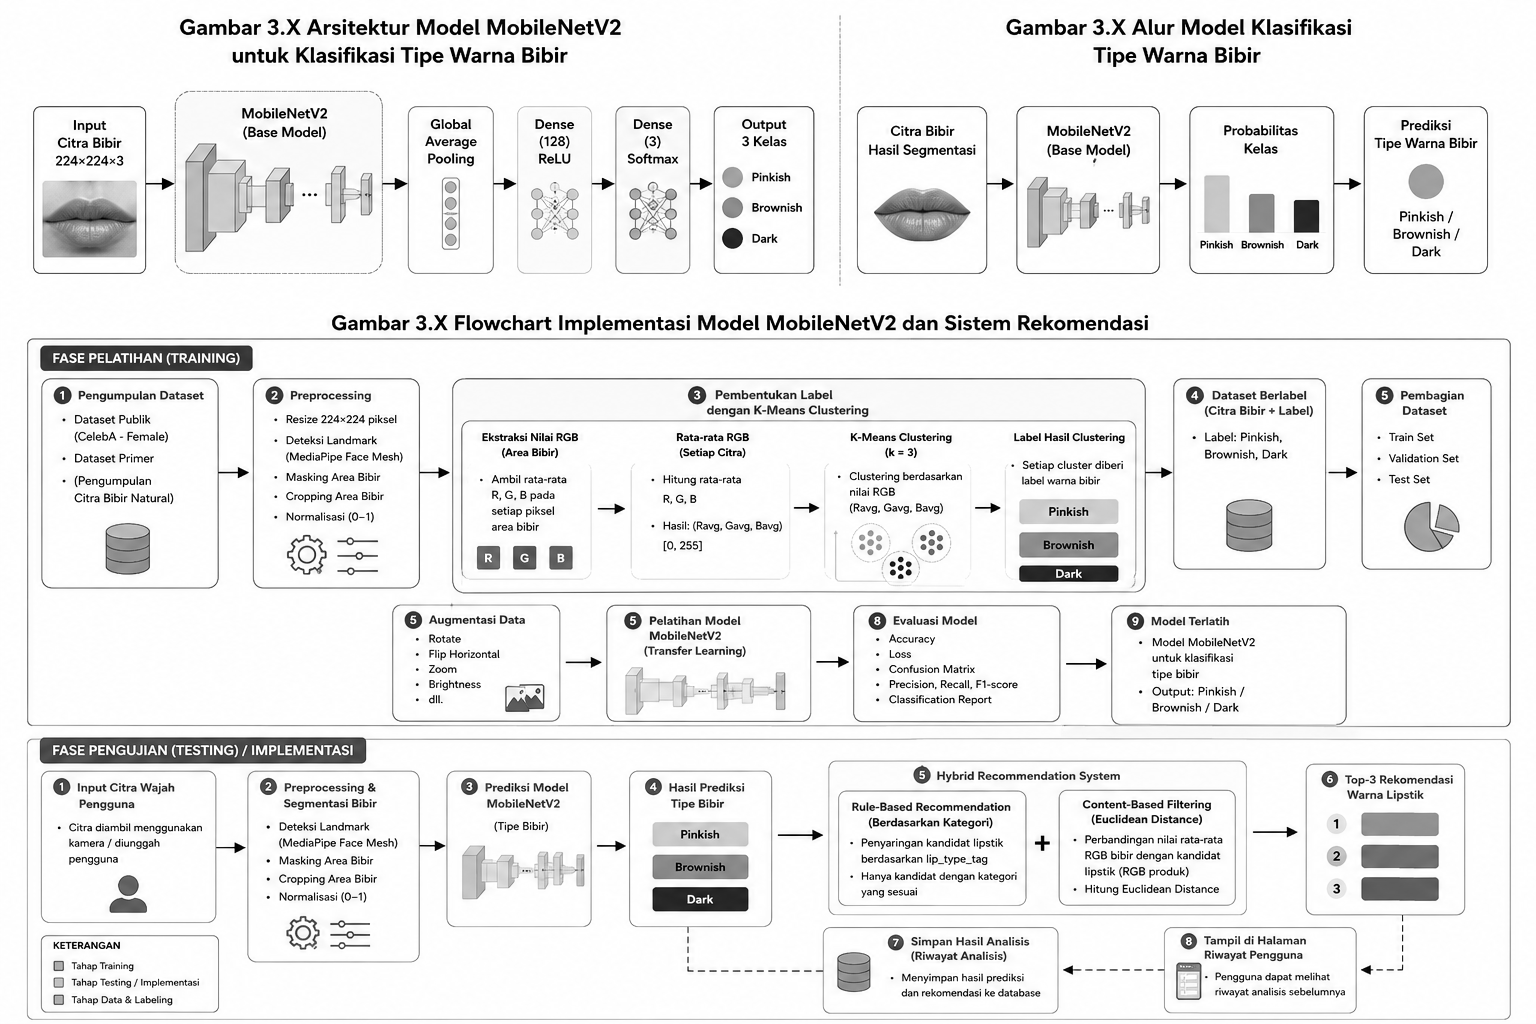
\includegraphics[width=0.72\textwidth]{skripsi_image28_bw.png}}{\fbox{System Flowchart Diagram}}
  \caption{System Architecture and Flowchart of Lipstick Shade Recommendation Using MobileNetV2 and Hybrid Recommendation System}
  \label{fig:alur_sistem}
\end{figure}

\subsection{Dataset Collection and Partitioning}
The dataset utilized in this research comprises a total of 18,100 facial images, consisting of:
\begin{enumerate}
    \item Secondary Dataset (CelebA): 18,000 facial images sourced from the CelebFaces Attributes Dataset (CelebA) \cite{liu2015deep} featuring neutral expressions without heavy lip makeup.
    \item Primary Dataset: 100 facial images of Indonesian women captured without lip makeup to enhance the representation of local lip pigmentation diversity.
\end{enumerate}
The complete dataset was partitioned into a training set of 14,480 images (80\%) and a validation set of 3,620 images (20\%) for model training and hyperparameter evaluation.

\subsection{Preprocessing and Lip Region Segmentation}
The preprocessing stage aims to isolate the Region of Interest (ROI) corresponding to the lip area and standardize image dimensions:
\begin{enumerate}
    \item Image Resizing: Standardizing input images to $224 \times 224$ pixels using OpenCV \cite{bradski2000opencv}.
    \item Facial Landmark Detection: Employing the MediaPipe Face Mesh framework to extract 468 3D facial landmark coordinates \cite{lugaresi2019mediapipe}. Outer and inner lip contours are precisely delineated (Figure \ref{fig:landmark_seg}(a)).
    \item Segmentation and Masking: Constructing a binary polygon mask based on digital image segmentation principles \cite{otsu1979threshold, gonzalez2018digital} derived from the lip boundary coordinates. All pixels outside the designated lip contour are set to zero (Figure \ref{fig:landmark_seg}(b)).
    \item Normalization and ROI Cropping: Rescaling RGB pixel intensities to the $[0, 1]$ interval and cropping the image tightly bounded by the lip coordinates ($x_{\min}, y_{\min}, x_{\max}, y_{\max}$).
\end{enumerate}

\begin{figure}[htbp]
  \centering
  \begin{subfigure}[b]{0.46\textwidth}
    \centering
    \IfFileExists{Gambar/skripsi_image39.png}{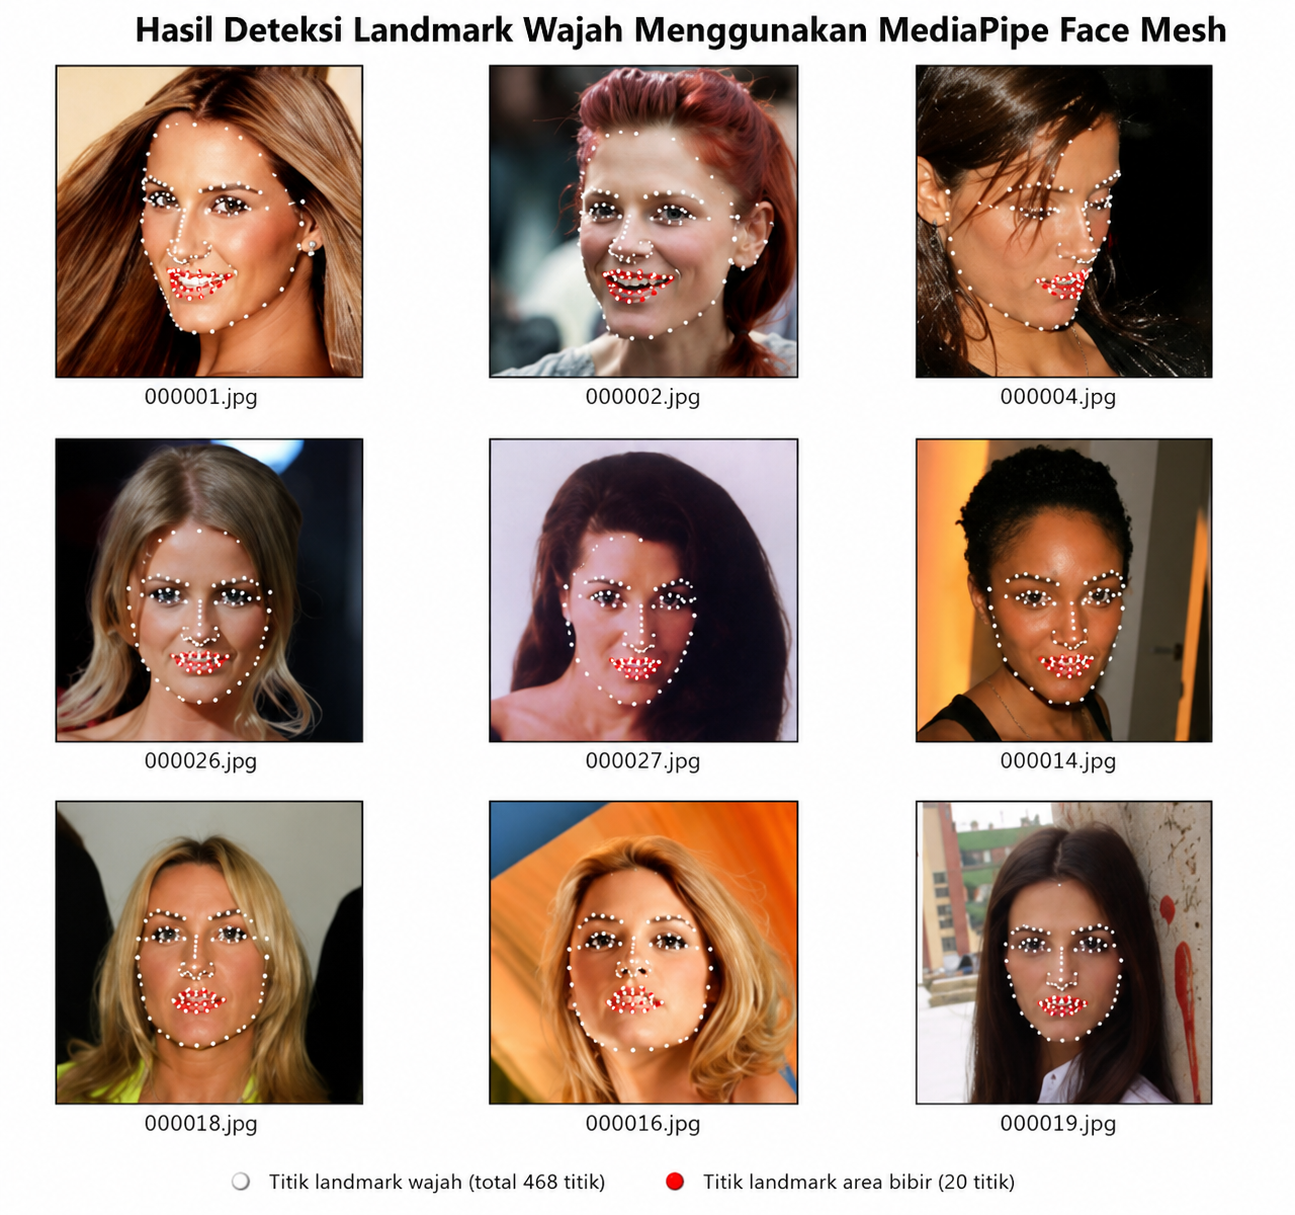
\includegraphics[width=\textwidth]{skripsi_image39.png}}{\fbox{Facial Landmarks}}
    \caption{MediaPipe Landmark Detection}
    \label{fig:landmark}
  \end{subfigure}
  \hfill
  \begin{subfigure}[b]{0.46\textwidth}
    \centering
    \IfFileExists{Gambar/skripsi_image40.png}{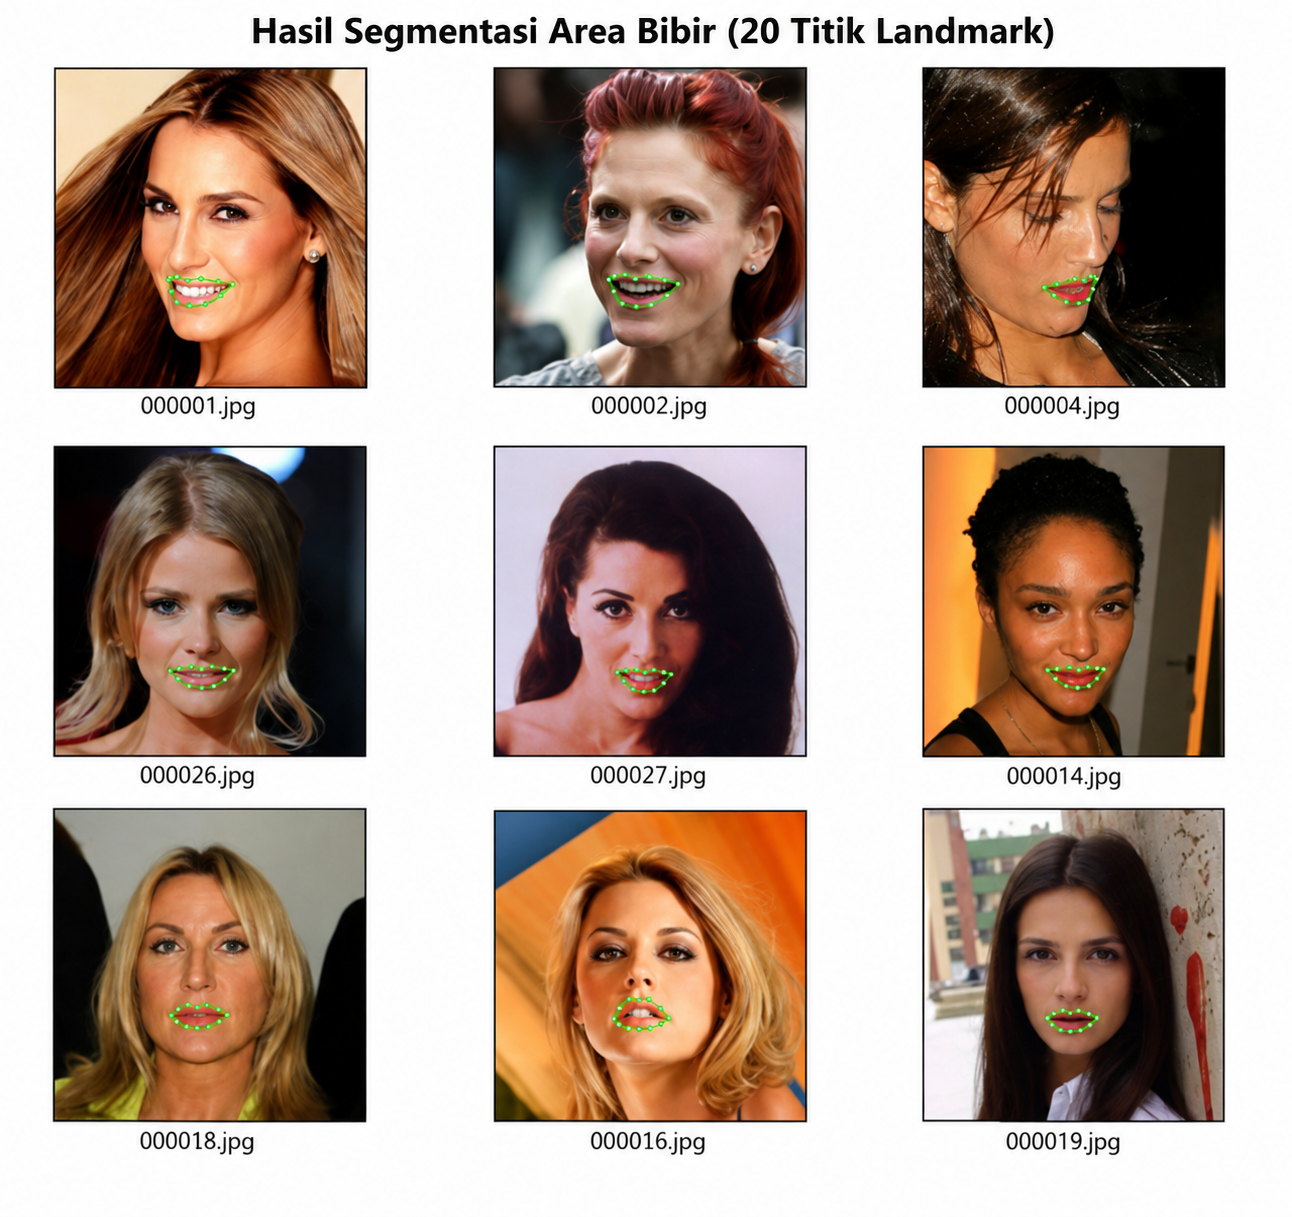
\includegraphics[width=\textwidth]{skripsi_image40.png}}{\fbox{Lip Segmentation}}
    \caption{Lip Segmentation and Masking}
    \label{fig:seg_bibir}
  \end{subfigure}
  \caption{Stages of Facial Landmark Detection and User Lip Region Segmentation}
  \label{fig:landmark_seg}
\end{figure}

\subsection{Color Feature Extraction and K-Means Clustering}
Lip color characteristics are extracted from the mean intensities of the Red ($R$), Green ($G$), and Blue ($B$) color channels across all $N$ segmented lip mask pixels using the formulation:
\begin{equation}
  \bar{R} = \frac{1}{N} \sum_{i=1}^N R_i, \quad \bar{G} = \frac{1}{N} \sum_{i=1}^N G_i, \quad \bar{B} = \frac{1}{N} \sum_{i=1}^N B_i
  \label{eq:rgb_avg}
\end{equation}

These three scalar values $(\bar{R}, \bar{G}, \bar{B})$ serve as input features to the K-Means Clustering algorithm ($K=3$, initialization \textit{k-means++}, random state 42) to establish three distinct natural lip type clusters (Figure \ref{fig:kmeans_viz}):
\begin{enumerate}
    \item Pinkish: Bright tones with dominant reddish or soft pink hue components ($\bar{R} > 150, \bar{G} \approx 95-120, \bar{B} \approx 100-125$).
    \item Brownish: Warm brownish tones ($\bar{R} \approx 125-155, \bar{G} \approx 75-100, \bar{B} \approx 65-90$).
    \item Dark: Lip tones characterized by deep, concentrated pigmentation ($\bar{R} < 110, \bar{G} < 65, \bar{B} < 60$).
\end{enumerate}

\begin{figure}[htbp]
  \centering
  \IfFileExists{Gambar/skripsi_image44.png}{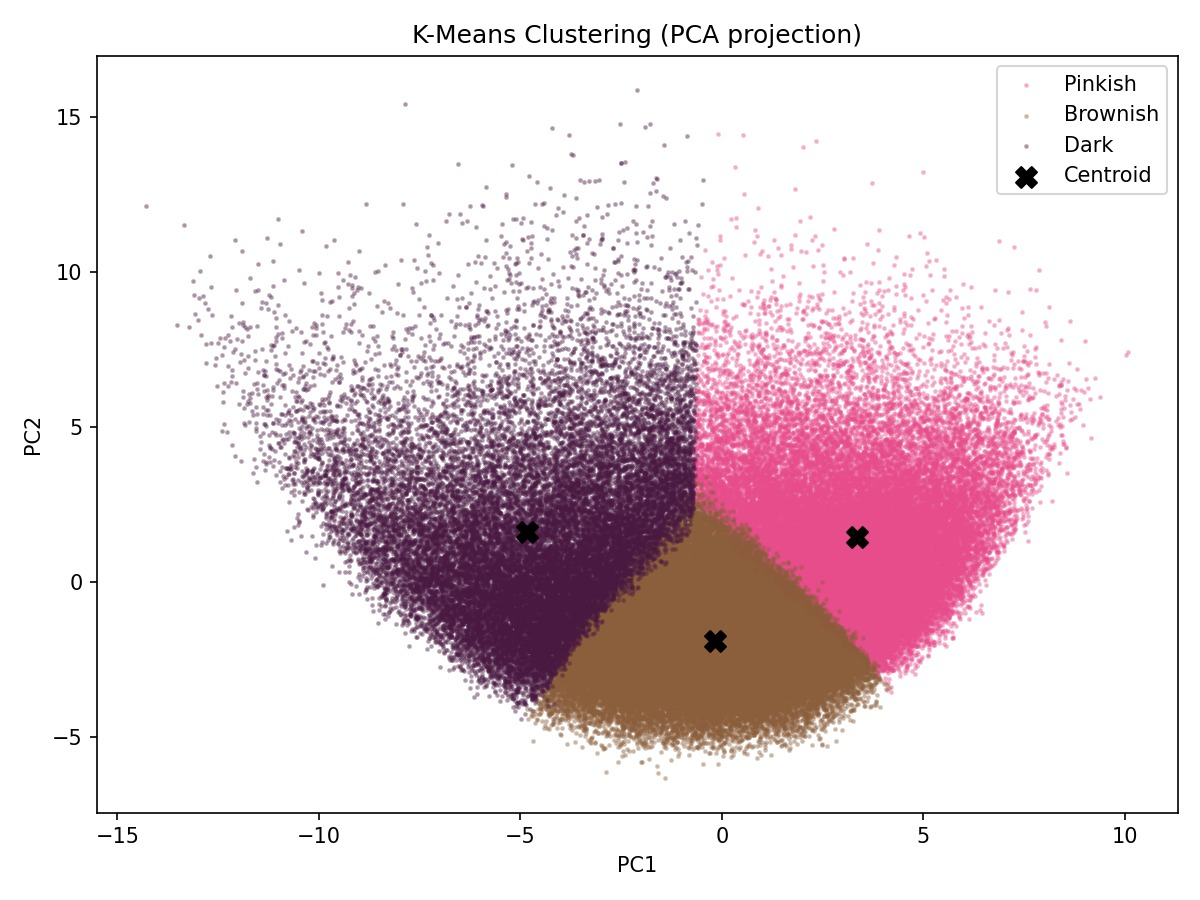
\includegraphics[width=0.48\textwidth]{skripsi_image44.png}}{\fbox{K-Means Visualization}}
  \caption{Distribution Visualization of Lip Color K-Means Clustering Results ($K=3$)}
  \label{fig:kmeans_viz}
\end{figure}

\subsection{MobileNetV2 Classification Model Training}
The MobileNetV2 architecture was trained using a Transfer Learning approach initialized with pre-trained ImageNet weights \cite{pan2010survey, he2016deep}, supported by image data augmentation techniques to broaden feature variability \cite{shorten2019survey}. Customized classification layers appended to the base feature extractor include: Global Average Pooling 2D, Dropout (0.3), Dense (128 units, ReLU activation), Dropout (0.2), and Dense Output (3 units, Softmax activation). The training hyperparameter configuration is summarized in Table \ref{tab:param_pelatihan}.

\begin{table}[htbp]
  \centering
  \caption{Hyperparameter Configuration for MobileNetV2 Model Training}
  \label{tab:param_pelatihan}
  \fontsize{8.5pt}{11pt}\selectfont
  \begin{tabular}{ll}
    \toprule
    \textbf{Parameter} & \textbf{Value / Configuration} \\
    \midrule
    Base Architecture & MobileNetV2 (ImageNet Pre-trained) \\
    Input Image Dimensions & $224 \times 224 \times 3$ pixels \\
    Number of Epochs & 30 \\
    Batch Size & 32 \\
    Optimizer & Adam ($\beta_1=0.9, \beta_2=0.999$, $\text{lr}=0.0001$) \\
    Loss Function & Categorical Crossentropy \\
    Number of Output Classes & 3 (Pinkish, Brownish, Dark) \\
    \bottomrule
  \end{tabular}
\end{table}

\subsection{Hybrid Recommendation System}
Once the MobileNetV2 classifier computes class probabilities for the user's lip tone ($\hat{y}_{\text{user}} \in \{\text{Pinkish}, \text{Brownish}, \text{Dark}\}$), the system identifies the most suitable lipstick shades through a two-stage hybrid mechanism:

\subsubsection{Stage 1: Rule-Based Filtering}
The system filters 281 commercial lipstick shades stored in the knowledge base by matching the \texttt{lip\_type\_tag} attribute with the user's predicted category:
\begin{equation}
  \mathcal{C}_{\text{candidate}} = \{ L_j \in \mathcal{D}_{\text{lipstick}} \mid \text{tag}(L_j) = \hat{y}_{\text{user}} \}
\end{equation}
The resulting candidate pool comprises 147 products for Pinkish, 127 products for Brownish, and 14 products for Dark categories (Table \ref{tab:rule_based}).

\begin{table}[htbp]
  \centering
  \caption{Rule-Based Recommendation Filtering Criteria Based on Lip Color Type}
  \label{tab:rule_based}
  \fontsize{8.5pt}{11pt}\selectfont
  \begin{tabular}{cllc}
    \toprule
    \textbf{No} & \textbf{Predicted Lip Color Type} & \textbf{Knowledge Base Filtering Criteria} & \textbf{Candidate Product Count} \\
    \midrule
    1 & Pinkish  & \texttt{lip\_type\_tag} = \textit{Pinkish}  & 147 products \\
    2 & Brownish & \texttt{lip\_type\_tag} = \textit{Brownish} & 127 products \\
    3 & Dark     & \texttt{lip\_type\_tag} = \textit{Dark}     & 14 products \\
    \midrule
    \multicolumn{3}{l}{\textbf{Total Lipstick Database Entries}} & \textbf{281 products} \\
    \bottomrule
  \end{tabular}
\end{table}

\subsubsection{Stage 2: Content-Based Filtering Using Euclidean Distance}
The system computes the geometric RGB color space distance (Euclidean Distance) between the user's lip color vector $\mathbf{u} = (R_u, G_u, B_u)$ and candidate lipstick shades $\mathbf{v}_j = (R_j, G_j, B_j)$ across all candidate items $L_j \in \mathcal{C}_{\text{candidate}}$:
\begin{equation}
  d(\mathbf{u}, \mathbf{v}_j) = \sqrt{(R_u - R_j)^2 + (G_u - G_j)^2 + (B_u - B_j)^2}
  \label{eq:euclidean}
\end{equation}

The geometric distance is then mapped to a percentage similarity score relative to the maximum diagonal span of the RGB color cube $d_{\max} = \sqrt{3 \times 255^2} \approx 441.673$:
\begin{equation}
  \text{Similarity}(\mathbf{u}, \mathbf{v}_j) = \left( 1 - \frac{d(\mathbf{u}, \mathbf{v}_j)}{d_{\max}} \right) \times 100\%
  \label{eq:similarity}
\end{equation}

The top three candidate products yielding the highest similarity scores are designated as the \textbf{Top-3 Lipstick Recommendation} (Algorithm \ref{alg:hybrid}).

\begin{algorithm}[htbp]
\caption{Hybrid Recommendation System Algorithm for Lipstick Shade Recommendation}
\label{alg:hybrid}
\fontsize{8.5pt}{10.5pt}\selectfont
\begin{algorithmic}[1]
\Require User facial image $I_{\text{face}}$, Lipstick product database $\mathcal{D}_{\text{lipstick}}$, MobileNetV2 classification model $\mathcal{M}$.
\Ensure Top-3 lipstick shade recommendations along with calculated percentage similarity scores.
\State $I_{\text{lip}} \gets \text{SegmentLipRegion}(I_{\text{face}})$ \Comment{MediaPipe Face Mesh segmentation}
\State $(R_u, G_u, B_u) \gets \text{ExtractAverageRGB}(I_{\text{lip}})$
\State $\hat{y}_{\text{user}} \gets \mathcal{M}.\text{predict}(I_{\text{lip}})$ \Comment{Classification: Pinkish, Brownish, or Dark}
\State $\mathcal{C}_{\text{candidate}} \gets \emptyset$
\For{each $L_j \in \mathcal{D}_{\text{lipstick}}$} \Comment{Stage 1: Rule-Based Filtering}
    \If{$L_j.\text{tag} == \hat{y}_{\text{user}}$}
        \State $\mathcal{C}_{\text{candidate}} \gets \mathcal{C}_{\text{candidate}} \cup \{L_j\}$
    \EndIf
\EndFor
\State $\mathcal{R} \gets []$
\For{each $L_j \in \mathcal{C}_{\text{candidate}}$} \Comment{Stage 2: Content-Based Filtering}
    \State $(R_j, G_j, B_j) \gets L_j.\text{rgb}$
    \State $d_j \gets \sqrt{(R_u - R_j)^2 + (G_u - G_j)^2 + (B_u - B_j)^2}$
    \State $S_j \gets (1 - d_j / 441.673) \times 100\%$
    \State Append $(L_j, d_j, S_j)$ to $\mathcal{R}$
\EndFor
\State Sort $\mathcal{R}$ in ascending order by distance $d_j$
\State \Return Top-3 elements of $\mathcal{R}$
\end{algorithmic}
\end{algorithm}

\subsection{Performance Evaluation Metrics}
Classification performance is evaluated using the Confusion Matrix and standard metrics: Accuracy, Precision, Recall, and F1-Score \cite{powers2011evaluation}:
\begin{equation}
  \text{Accuracy} = \frac{TP + TN}{TP + TN + FP + FN}
\end{equation}
\begin{equation}
  \text{Precision} = \frac{TP}{TP + FP}, \quad \text{Recall} = \frac{TP}{TP + FN}, \quad \text{F1-Score} = 2 \times \frac{\text{Precision} \times \text{Recall}}{\text{Precision} + \text{Recall}}
\end{equation}

% =========================================================================
% Section 3: Results and Discussion
% =========================================================================
\section{RESULTS AND DISCUSSION}

\subsection{MobileNetV2 Model Training and Evaluation Results}
The MobileNetV2 architecture was trained for 30 epochs on the dataset annotated via K-Means clustering. Figure \ref{fig:eval_mobilenet}(a) depicts the convergence curves of accuracy and categorical loss, while Figure \ref{fig:eval_mobilenet}(b) displays the resulting Confusion Matrix evaluated on the validation dataset (803 samples).

\begin{figure}[htbp]
  \centering
  \begin{subfigure}[b]{0.52\textwidth}
    \centering
    \IfFileExists{Gambar/skripsi_image45.png}{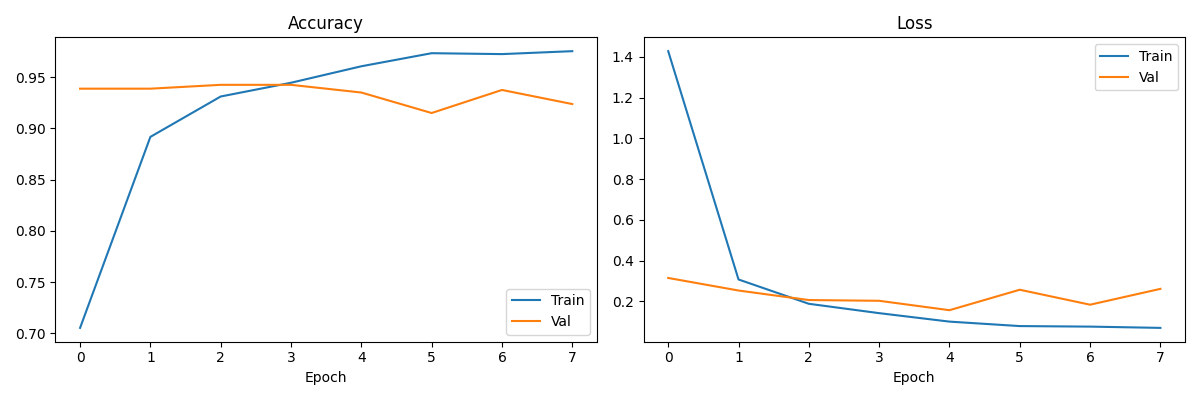
\includegraphics[width=\textwidth]{skripsi_image45.png}}{\fbox{Accuracy and Loss Graph}}
    \caption{Training Accuracy and Loss Graph}
    \label{fig:loss_acc}
  \end{subfigure}
  \hfill
  \begin{subfigure}[b]{0.44\textwidth}
    \centering
    \IfFileExists{Gambar/skripsi_image46.png}{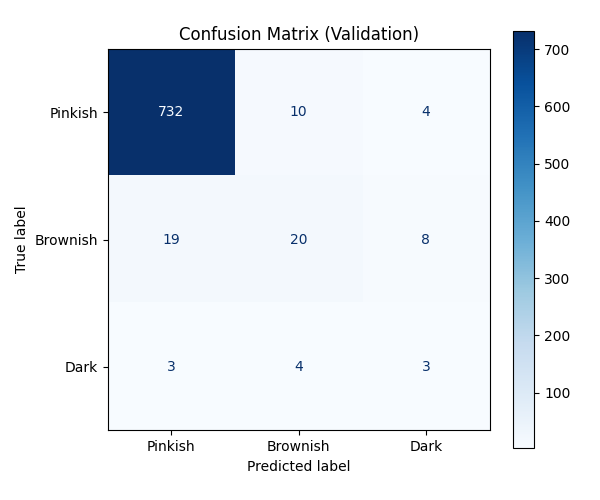
\includegraphics[width=\textwidth]{skripsi_image46.png}}{\fbox{Confusion Matrix}}
    \caption{Validation Confusion Matrix}
    \label{fig:cm}
  \end{subfigure}
  \caption{MobileNetV2 Performance Evaluation: (a) Accuracy and Loss Convergence Graph, (b) Confusion Matrix on Validation Data}
  \label{fig:eval_mobilenet}
\end{figure}

The model attained stable convergence beyond the 15th epoch without indications of overfitting, yielding a final validation accuracy of \textbf{94.84\%} and a validation loss of \textbf{0.1612}. Detailed performance metrics across individual classes are summarized in the Classification Report in Table \ref{tab:classification_report}.

\begin{table}[htbp]
  \centering
  \caption{MobileNetV2 Model Performance Classification Report}
  \label{tab:classification_report}
  \fontsize{8.5pt}{11pt}\selectfont
  \begin{tabular}{lcccc}
    \toprule
    \textbf{Lip Tone Class} & \textbf{Precision} & \textbf{Recall} & \textbf{F1-Score} & \textbf{Support (Samples)} \\
    \midrule
    Pinkish      & 0.971 (97.1\%) & 0.981 (98.1\%) & 0.976 (97.6\%) & 746 \\
    Brownish     & 0.588 (58.8\%) & 0.426 (42.6\%) & 0.494 (49.4\%) & 47  \\
    Dark         & 0.200 (20.0\%) & 0.300 (30.0\%) & 0.240 (24.0\%) & 10  \\
    \midrule
    \textbf{Overall Accuracy} & \multicolumn{3}{c}{\textbf{0.940 (94.0\%)}} & \textbf{803} \\
    \textbf{Macro Average}    & 0.586 & 0.569 & 0.570 & 803 \\
    \textbf{Weighted Average} & 0.939 & 0.940 & 0.938 & 803 \\
    \bottomrule
  \end{tabular}
\end{table}

The model demonstrates strong predictive performance on the \textbf{Pinkish} class (F1-score 97.6\%). On the \textbf{Brownish} and \textbf{Dark} classes, F1-scores were 49.4\% and 24.0\%, respectively. These values reflect the predominance of lighter lip tones within the public facial dataset (\textit{class imbalance}). Nevertheless, across all samples, the model achieved a weighted average F1-score of 93.8\% and an overall accuracy of 94.0\%, validating MobileNetV2's effectiveness in recognizing lip visual characteristics.

\subsection{Testing and Evaluation of the Hybrid Recommendation System}
Evaluation of the recommendation system was conducted using 30 user test samples with diverse lip RGB color values. Selected sample test outputs are presented in Table \ref{tab:hasil_rekomendasi}, and the overall quantitative summary is detailed in Table \ref{tab:rekap_similarity}.

\begin{table}[htbp]
  \centering
  \caption{Sample Results of the Hybrid Recommendation System on User Test Data}
  \label{tab:hasil_rekomendasi}
  \fontsize{8.5pt}{10.5pt}\selectfont
  \begin{tabular}{ccclccc}
    \toprule
    \textbf{No} & \textbf{User RGB} & \textbf{Lip Type} & \textbf{Shade Recommendation} & \textbf{Lipstick RGB} & \textbf{Euclidean ($d$)} & \textbf{Similarity (\%)} \\
    \midrule
    1 & (164, 121, 108) & Pinkish  & 1. Glossy Berry     & (167, 97, 101)  & 25.18 & 94.3\% \\
      &                 &          & 2. Dusty Rose       & (185, 115, 125) & 27.68 & 93.7\% \\
      &                 &          & 3. Cozy Cherry      & (173, 98, 94)   & 28.39 & 93.6\% \\
    \midrule
    2 & (128, 102, 99)  & Brownish & 1. Chilled Raspberry& (134, 85, 109)  & 20.62 & 95.3\% \\
      &                 &          & 2. Chilled Cranberry& (132, 68, 82)   & 38.22 & 91.3\% \\
      &                 &          & 3. Matte Berry      & (162, 83, 86)   & 41.06 & 90.7\% \\
    \midrule
    3 & (145, 98, 55)   & Pinkish  & 1. Satin Vermillion & (173, 95, 86)   & 41.88 & 90.5\% \\
      &                 &          & 2. Bold Ruby        & (176, 88, 86)   & 44.97 & 89.8\% \\
      &                 &          & 3. Cozy Cherry      & (173, 98, 94)   & 48.01 & 89.1\% \\
    \midrule
    4 & (195, 167, 153) & Brownish & 1. Mauve Bliss      & (170, 110, 130) & 66.36 & 85.0\% \\
      &                 &          & 2. Warm Terracotta  & (180, 105, 95)  & 74.35 & 83.2\% \\
      &                 &          & 3. Rose Brown       & (160, 95, 110)  & 81.12 & 81.6\% \\
    \bottomrule
  \end{tabular}
\end{table}

\begin{table}[htbp]
  \centering
  \caption{Quantitative Summary of Similarity Scores for the Hybrid Recommendation System}
  \label{tab:rekap_similarity}
  \fontsize{8.5pt}{11pt}\selectfont
  \begin{tabular}{lc}
    \toprule
    \textbf{Evaluation Metric} & \textbf{Quantitative Value} \\
    \midrule
    Number of Evaluation Test Samples & 30 data points \\
    Average Top-1 Similarity (First Recommendation)  & \textbf{93.62\%} \\
    Average Top-2 Similarity (Second Recommendation) & \textbf{92.26\%} \\
    Average Top-3 Similarity (Third Recommendation)  & \textbf{91.41\%} \\
    Highest Recorded Similarity Score                & \textbf{97.60\%} \\
    Lowest Recorded Similarity Score                 & \textbf{73.60\%} \\
    Total Registered Commercial Lipstick Shades      & 281 shades \\
    \bottomrule
  \end{tabular}
\end{table}

The performance summary demonstrates that the hybrid recommendation system consistently produces lipstick shade recommendations with high compatibility. The average color similarity for the primary recommendation (Top-1) reached \textbf{93.62\%}, with all Top-3 recommendations consistently exceeding 91\%. The two-stage hybrid framework proves effective in filtering out mismatched categories during the Rule-Based phase while maximizing fine-grained color gradation matching during the Euclidean Distance stage.

\subsection{Web-Based System User Interface Implementation}
The system was deployed as a responsive web application. Users upload a facial photograph, after which the application automatically displays the segmented lip ROI, extracted RGB values, MobileNetV2 predicted classification, confidence score, and interactive Top-3 recommendation cards complete with color swatches and similarity percentages (Figure \ref{fig:ui_analisis}).

\begin{figure}[htbp]
  \centering
  \IfFileExists{Gambar/skripsi_image34.png}{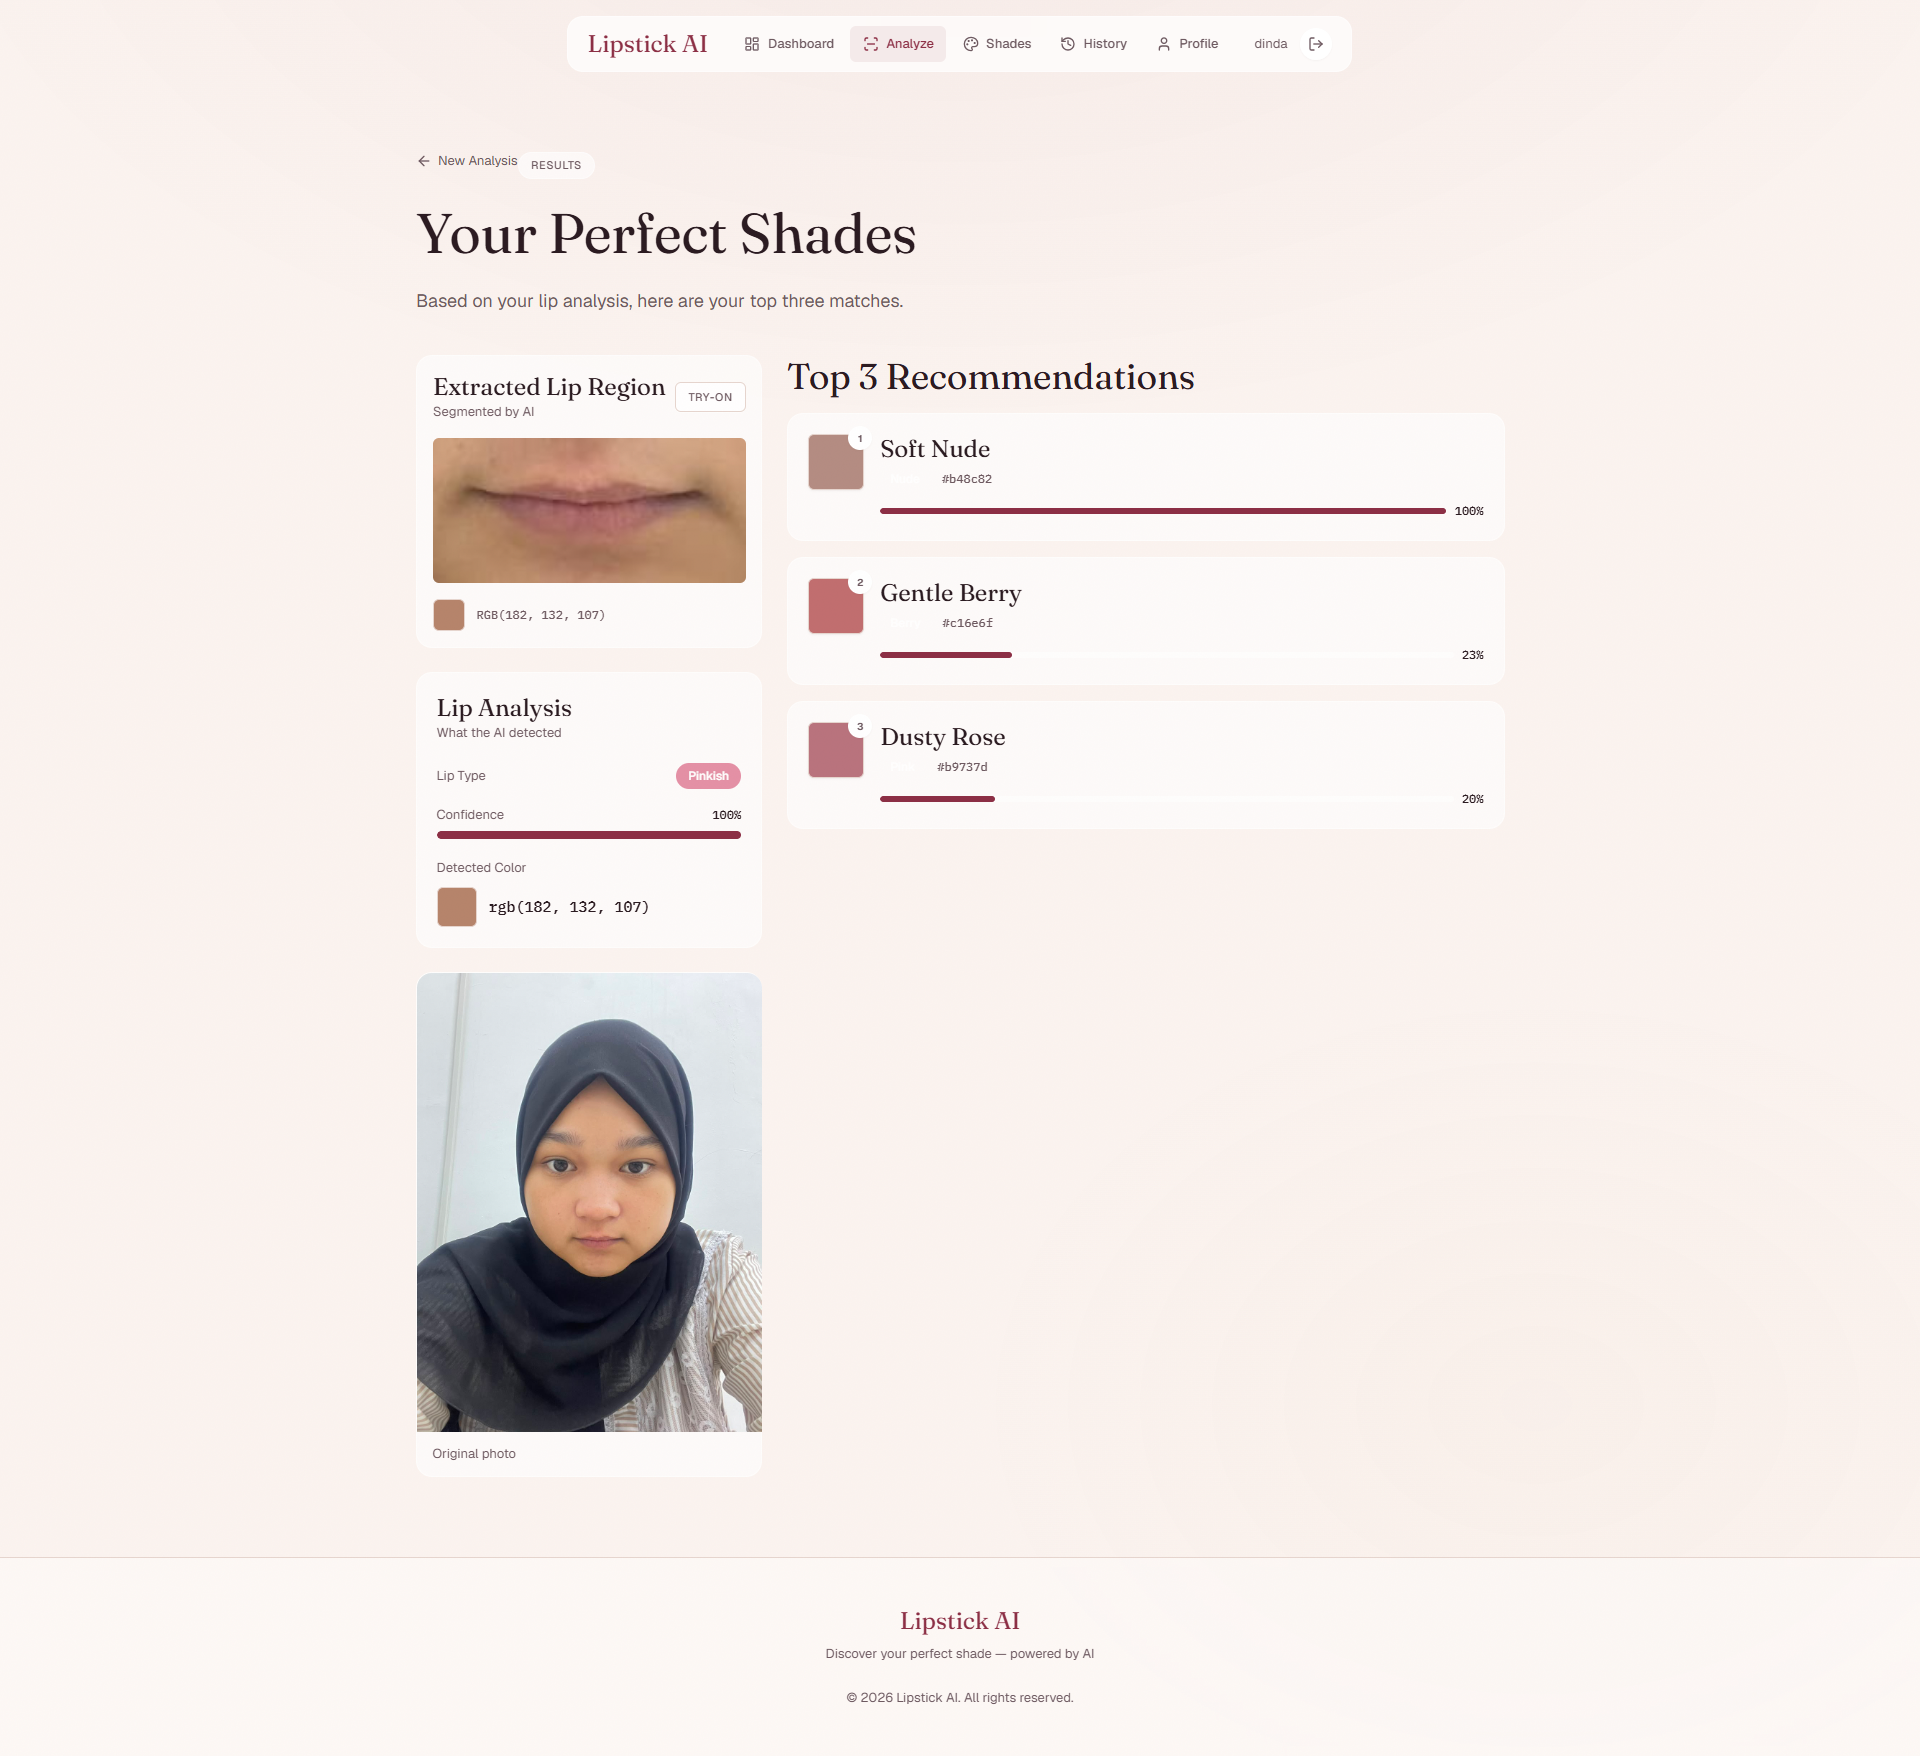
\includegraphics[width=0.55\textwidth]{skripsi_image34.png}}{\fbox{Analysis Results Interface}}
  \caption{User Interface Implementation of Analysis Results and Lipstick Recommendations}
  \label{fig:ui_analisis}
\end{figure}

\subsection{Functional Testing (Black Box Testing)}
Functional evaluation using Black Box Testing verified that all core software modules operate according to operational requirements, achieving a \textbf{100\% PASS} rate (Table \ref{tab:blackbox}).

\begin{table}[htbp]
  \centering
  \caption{Black Box Testing Results for Analysis and Recommendation Modules}
  \label{tab:blackbox}
  \fontsize{8pt}{10pt}\selectfont
  \begin{tabularx}{\textwidth}{clXXc}
    \toprule
    \textbf{No} & \textbf{Test Scenario} & \textbf{Activity / Input} & \textbf{Expected Output} & \textbf{Status} \\
    \midrule
    1 & Valid Image Upload     & JPG/PNG facial image & Face detected and image preview rendered & PASS \\
    2 & Landmark Detection     & Execute analysis & MediaPipe extracts 468 3D facial landmarks & PASS \\
    3 & Lip Segmentation       & Delineate lip boundary & Polygon mask generated and lip region cropped & PASS \\
    4 & Color Classification   & RGB extraction \& inference & MobileNetV2 predicts class (Pinkish/Brownish/Dark) & PASS \\
    5 & Top-3 Recommendation   & Rule filter \& Euclidean metric & Top 3 lipstick shades with highest similarity displayed & PASS \\
    6 & Save History           & Commit to database & Record persisted and retrievable via History menu & PASS \\
    \bottomrule
  \end{tabularx}
\end{table}

\FloatBarrier
% =========================================================================
% Section 4: Conclusion
% =========================================================================
\section{CONCLUSION AND FUTURE WORK}

\subsection{Conclusion}
Based on the design, development, and evaluation conducted, this study has successfully established an automated, personalized lip image-based lipstick shade recommendation system integrating MediaPipe Face Mesh, MobileNetV2 via transfer learning, and a Hybrid Recommendation System. The MobileNetV2 model proved reliable in classifying natural lip tones into three defined categories (Pinkish, Brownish, and Dark), achieving a validation accuracy of 94.84\% and a validation loss of 0.1612. Furthermore, integrating Rule-Based Filtering and Content-Based Filtering based on Euclidean Distance effectively optimized recommendation precision from a commercial cosmetic database, attaining average similarity scores of 93.62\% for the first recommendation, 92.26\% for the second recommendation, and 91.41\% for the third recommendation, with a peak compatibility score of 97.60\%. Functional validation through Black Box Testing verified that all application modules execute reliably with a 100\% success rate.

\subsection{Future Work}
For future research and system enhancement, increasing primary sample diversity—particularly within the underrepresented Dark and Brownish pigmentation categories—is recommended. Incorporating specialized class imbalance countermeasures such as class weighting or SMOTE will further enhance minority class sensitivity. Additionally, subsequent developments may extend system functionality by introducing interactive Augmented Reality (AR) Virtual Try-On capabilities, as well as integrating skin undertone and occasion-based preferences to deliver even more comprehensive and adaptive cosmetic recommendations.

% =========================================================================
% References (IEEE Style)
% =========================================================================
\section*{REFERENCES}

\begingroup
\renewcommand{\section}[2]{}%
\begin{thebibliography}{99}
\fontsize{8pt}{10pt}\selectfont
\setlength{\itemsep}{2pt}
\setlength{\parskip}{0pt}

\bibitem{jakpat2025}
Jakpat Survey, 2025, ``Makeup Product Categories Used by Indonesian Women in 2025,'' \textit{Databoks Katadata}, Katadata Indonesia, URL: \url{https://databoks.katadata.co.id/en/consumer-durables-apparel/statistics/692e89e11c6f5/makeup-product-categories-used-by-indonesian-women-in-2025}, Abstract: Survey on cosmetic usage showing lip products as the most popular category used by Indonesian women (80.4\%)., Keywords: Makeup categories, Indonesian women, Cosmetics market, Lip products, Document Type: Online Report, Language: English, Database/Indexing: Katadata Databoks, Citation Key: \texttt{jakpat2025}.

\bibitem{vergnaud2024lip}
H. Vergnaud, Z. Charton, D. Blumenthal, V. Couturaud, M. Le Fur, E. Loescher, et al., 2024, ``Lip Color Diversity: An Intricate Study,'' \textit{Skin Research and Technology}, vol. 30, no. 2, p. e13583, John Wiley \& Sons, Inc., doi: 10.1111/srt.13583, ISSN: 1600-0846, URL: \url{https://doi.org/10.1111/srt.13583}, Abstract: Analysis of multi-ethnic lip pigmentation variations and underlying anatomical and physiological factors., Keywords: Lip color diversity, Melanin, Hemoglobin, Ethnicity, Skin colorimetry, Document Type: Journal Article, Language: English, Database/Indexing: Scopus / PubMed, Citation Key: \texttt{vergnaud2024lip}.

\bibitem{vergnaud2023measurement}
H. Vergnaud, M. Cherel, G. Fran\c{c}ois, Z. Charton, E. Loescher, L. Caisey, et al., 2023, ``Lip Color Measurement: A New Hyperspectral Imaging Device,'' \textit{Skin Research and Technology}, vol. 29, no. 8, p. e13418, John Wiley \& Sons, Inc., doi: 10.1111/srt.13418, ISSN: 1600-0846, URL: \url{https://doi.org/10.1111/srt.13418}, Abstract: Introduction of a hyperspectral imaging methodology for high-fidelity non-contact measurement of human lip color., Keywords: Lip color measurement, Hyperspectral imaging, Colorimetry, Spectroscopy, Document Type: Journal Article, Language: English, Database/Indexing: Scopus / PubMed, Citation Key: \texttt{vergnaud2023measurement}.

\bibitem{charton2026development}
Z. Charton, H. Vergnaud, L. Caisey, D. Blumenthal, M. Ma, A. Shi, et al., 2026, ``Development of a Lip Colour Chart Across Four Ethnicities,'' \textit{International Journal of Cosmetic Science}, vol. 48, no. 1, pp. 161--171, John Wiley \& Sons, Inc., doi: 10.1111/ics.70004, ISSN: 0142-5463, URL: \url{https://doi.org/10.1111/ics.70004}, Abstract: Construction of standardized multi-ethnic lip color chart aiding cosmetic product formulation and shade matching., Keywords: Lip colour chart, Multi-ethnic shade matching, Cosmetic science, Spectrophotometry, Document Type: Journal Article, Language: English, Database/Indexing: Scopus / Wiley Online Library, Citation Key: \texttt{charton2026development}.

\bibitem{katariya2025novel}
R. Katariya and S. Patel, 2025, ``A Novel Strid CNN Model for Cosmetic Product Recommendation based on Skin Type and Tone,'' \textit{SSRG International Journal of Electrical and Electronics Engineering}, vol. 12, no. 5, pp. 1--12, Seventh Sense Research Group, doi: 10.14445/23488379/IJEEE-V12I5P101, ISSN: 2348-8379, URL: \url{https://doi.org/10.14445/23488379/IJEEE-V12I5P101}, Abstract: Application of custom convolutional neural network for classifying skin types and predicting cosmetic products., Keywords: Cosmetic recommendation, Skin tone classification, Convolutional neural networks, Computer vision, Document Type: Journal Article, Language: English, Database/Indexing: SSRG / Google Scholar, Citation Key: \texttt{katariya2025novel}.

\bibitem{gulati2023beautifai}
K. Gulati, G. Verma, M. Mohania, and A. Kundu, 2023, ``BeautifAI: Personalised Occasion-based Makeup Recommendation,'' \textit{Proc. 14th Asian Conf. Mach. Learn. (ACML), PMLR}, vol. 189, pp. 407--419, PMLR, ISSN: 2640-3498, URL: \url{https://proceedings.mlr.press/v189/gulati23a.html}, Abstract: Machine learning framework recommending personalized makeup looks matching occasion and user facial traits., Keywords: Makeup recommendation, Facial cosmetics, Occasion-based styling, Deep learning, Document Type: Conference Paper, Language: English, Database/Indexing: PMLR / DBLP, Citation Key: \texttt{gulati2023beautifai}.

\bibitem{pratama2025sistem}
R. Pratama et al., 2025, ``Sistem Rekomendasi Produk Kosmetik Menggunakan Metode Content-Based Filtering Berbasis Website,'' \textit{Jurnal Rabit: Jurnal Teknologi dan Sistem Informasi Univ. Abdurrab}, vol. 10, no. 1, pp. 45--56, Universitas Abdurrab, ISSN: 2477-2062, URL: \url{https://jurnal.univrab.ac.id/index.php/rabit/article/view/6371}, Abstract: Web-based cosmetic recommendation system implementation applying Euclidean distance content-based filtering., Keywords: Content-based filtering, Euclidean distance, Cosmetics recommendation, Web system, Document Type: Journal Article, Language: Indonesian, Database/Indexing: SINTA / Garuda, Citation Key: \texttt{pratama2025sistem}.

\bibitem{szeliski2022computer}
R. Szeliski, 2022, ``Computer Vision: Algorithms and Applications,'' \textit{Springer Nature}, 2nd ed., Springer Cham, doi: 10.1007/978-3-030-34372-9, ISSN: 1868-0941, URL: \url{https://doi.org/10.1007/978-3-030-34372-9}, Abstract: Foundational textbook on fundamental computer vision algorithms, modern deep learning architectures, and applications., Keywords: Computer vision, Image classification, Recognition, Feature representation, Document Type: Book, Language: English, Database/Indexing: SpringerLink, Citation Key: \texttt{szeliski2022computer}.

\bibitem{goodfellow2016deep}
I. Goodfellow, Y. Bengio, and A. Courville, 2016, ``Deep Learning,'' \textit{MIT Press}, MIT Press, ISSN: 978-0262035613, URL: \url{https://www.deeplearningbook.org/}, Abstract: Authoritative reference on deep feedforward networks, regularization, optimization, and convolutional networks., Keywords: Deep learning, Neural networks, Convolutional networks, Optimization, Document Type: Book, Language: English, Database/Indexing: MIT Press, Citation Key: \texttt{goodfellow2016deep}.

\bibitem{lecun2015deep}
Y. LeCun, Y. Bengio, and G. Hinton, 2015, ``Deep Learning,'' \textit{Nature}, vol. 521, no. 7553, pp. 436--444, Nature Publishing Group, doi: 10.1038/nature14539, ISSN: 0028-0836, URL: \url{https://doi.org/10.1038/nature14539}, Abstract: Seminal review paper explaining foundations, capabilities, and future breakthroughs of deep learning in vision and speech., Keywords: Deep learning, Representation learning, Convolutional networks, Artificial intelligence, Document Type: Journal Article, Language: English, Database/Indexing: Scopus / Web of Science, Citation Key: \texttt{lecun2015deep}.

\bibitem{sandler2018mobilenetv2}
M. Sandler, A. Howard, M. Zhu, A. Zhmoginov, and L.-C. Chen, 2018, ``MobileNetV2: Inverted Residuals and Linear Bottlenecks,'' \textit{Proc. IEEE/CVF Conf. Comput. Vis. Pattern Recognit. (CVPR)}, pp. 4510--4520, IEEE, doi: 10.1109/CVPR.2018.00474, ISSN: 2575-7075, URL: \url{https://doi.org/10.1109/CVPR.2018.00474}, Abstract: Novel mobile neural network architecture utilizing inverted residual blocks with linear bottlenecks for efficient vision tasks., Keywords: MobileNetV2, Inverted residuals, Linear bottlenecks, Convolutional neural networks, Mobile vision, Document Type: Conference Paper, Language: English, Database/Indexing: IEEE Xplore / Scopus, Citation Key: \texttt{sandler2018mobilenetv2}.

\bibitem{howard2017mobilenets}
A. G. Howard, M. Zhu, B. Chen, D. Kalenichenko, W. Wang, T. Weyand, et al., 2017, ``MobileNets: Efficient Convolutional Neural Networks for Mobile Vision Applications,'' \textit{arXiv preprint arXiv:1704.04861}, arXiv, doi: 10.48550/arXiv.1704.04861, URL: \url{https://arxiv.org/abs/1704.04861}, Abstract: Introduction of depthwise separable convolutions to dramatically decrease parameter count and latency for mobile deep learning., Keywords: MobileNets, Depthwise separable convolution, Efficient CNN, Mobile vision, Document Type: Preprint, Language: English, Database/Indexing: arXiv, Citation Key: \texttt{howard2017mobilenets}.

\bibitem{macqueen1967methods}
J. MacQueen, 1967, ``Some Methods for Classification and Analysis of Multivariate Observations,'' \textit{Proc. 5th Berkeley Symp. Math. Statist. Prob.}, vol. 1, pp. 281--297, University of California Press, URL: \url{https://projecteuclid.org/euclid.bsmsp/1200512992}, Abstract: Original formulation of the k-means clustering process for iterative partitioning and minimum variance multivariate analysis., Keywords: K-Means clustering, Multivariate analysis, Unsupervised classification, Centroid optimization, Document Type: Conference Paper, Language: English, Database/Indexing: Project Euclid, Citation Key: \texttt{macqueen1967methods}.

\bibitem{pedregosa2011scikit}
F. Pedregosa, G. Varoquaux, A. Gramfort, V. Michel, B. Thirion, O. Grisel, et al., 2011, ``Scikit-learn: Machine Learning in Python,'' \textit{Journal of Machine Learning Research}, vol. 12, pp. 2825--2830, JMLR.org, ISSN: 1532-4435, URL: \url{https://jmlr.org/papers/v12/pedregosa11a.html}, Abstract: Python module integrating widely accessible, unified, and efficient machine learning algorithms for medium-scale problems., Keywords: Scikit-learn, Python, Machine learning, Data mining, Scientific computing, Document Type: Journal Article, Language: English, Database/Indexing: JMLR / Scopus, Citation Key: \texttt{pedregosa2011scikit}.

\bibitem{ricci2015recommender}
F. Ricci, L. Rokach, and B. Shapira, 2015, ``Recommender Systems Handbook,'' \textit{Springer}, 2nd ed., Springer New York, doi: 10.1007/978-1-4899-7637-6, ISSN: 978-1-4899-7636-9, URL: \url{https://doi.org/10.1007/978-1-4899-7637-6}, Abstract: Exhaustive reference handbook on content-based filtering, collaborative filtering, hybrid techniques, and evaluation., Keywords: Recommender systems, Hybrid recommendation, Content-based filtering, Collaborative filtering, Document Type: Book, Language: English, Database/Indexing: SpringerLink, Citation Key: \texttt{ricci2015recommender}.

\bibitem{aggarwal2016recommender}
C. C. Aggarwal, 2016, ``Recommender Systems: The Textbook,'' \textit{Springer Nature}, Springer Cham, doi: 10.1007/978-3-319-29659-3, ISSN: 978-3-319-29658-6, URL: \url{https://doi.org/10.1007/978-3-319-29659-3}, Abstract: Foundational textbook covering mathematical algorithms and applications of recommender systems and distance similarity metrics., Keywords: Recommender systems, Collaborative filtering, Content-based models, Similarity metrics, Document Type: Book, Language: English, Database/Indexing: SpringerLink, Citation Key: \texttt{aggarwal2016recommender}.

\bibitem{lugaresi2019mediapipe}
C. Lugaresi, J. Tang, H. Nash, C. McClanahan, E. Uboweja, M. Hays, et al., 2019, ``MediaPipe: A Framework for Building Perception Pipelines,'' \textit{arXiv preprint arXiv:1906.08172}, arXiv, URL: \url{https://arxiv.org/abs/1906.08172}, Abstract: Open-source modular framework enabling cross-platform streaming perception pipelines including 3D face mesh estimation., Keywords: MediaPipe, Real-time perception, Face mesh, Streaming pipelines, Mobile computer vision, Document Type: Preprint, Language: English, Database/Indexing: arXiv, Citation Key: \texttt{lugaresi2019mediapipe}.

\bibitem{liu2015deep}
Z. Liu, P. Luo, X. Wang, and X. Tang, 2015, ``Deep Learning Face Attributes in the Wild,'' \textit{Proc. IEEE Int. Conf. Comput. Vis. (ICCV)}, pp. 3730--3738, IEEE, doi: 10.1109/ICCV.2015.425, URL: \url{https://doi.org/10.1109/ICCV.2015.425}, Abstract: Establishment of CelebA large-scale benchmark dataset and deep cascaded neural networks for facial attribute prediction., Keywords: CelebA, Face attributes, Deep learning, Face localization, Facial representation, Document Type: Conference Paper, Language: English, Database/Indexing: IEEE Xplore / Scopus, Citation Key: \texttt{liu2015deep}.

\bibitem{bradski2000opencv}
G. Bradski, 2000, ``The OpenCV Library,'' \textit{Dr. Dobb's Journal of Software Tools}, vol. 25, no. 11, pp. 120--125, Miller Freeman Inc., ISSN: 1044-789X, Abstract: Design, capabilities, and computational architecture of OpenCV real-time computer vision library., Keywords: OpenCV, Computer vision library, Real-time image processing, C/C++, Document Type: Journal Article, Language: English, Database/Indexing: Scopus, Citation Key: \texttt{bradski2000opencv}.

\bibitem{otsu1979threshold}
N. Otsu, 1979, ``A Threshold Selection Method from Gray-Level Histograms,'' \textit{IEEE Transactions on Systems, Man, and Cybernetics}, vol. 9, no. 1, pp. 62--66, IEEE, doi: 10.1109/TSMC.1979.4310076, ISSN: 0018-9472, URL: \url{https://doi.org/10.1109/TSMC.1979.4310076}, Abstract: Classic non-parametric threshold selection technique maximizing discriminant between-class variance in image histograms., Keywords: Otsu thresholding, Image binarization, Gray-level histogram, Image segmentation, Document Type: Journal Article, Language: English, Database/Indexing: IEEE Xplore / Scopus, Citation Key: \texttt{otsu1979threshold}.

\bibitem{gonzalez2018digital}
R. C. Gonzalez and R. E. Woods, 2018, ``Digital Image Processing,'' \textit{Pearson Education Limited}, 4th ed., Pearson Education Limited, ISSN: 978-0133356724, Abstract: Comprehensive textbook covering spatial filtering, image restoration, color processing, segmentation, and feature extraction., Keywords: Digital image processing, Color spaces, Image segmentation, Feature extraction, Document Type: Book, Language: English, Database/Indexing: Google Books, Citation Key: \texttt{gonzalez2018digital}.

\bibitem{pan2010survey}
S. J. Pan and Q. Yang, 2010, ``A Survey on Transfer Learning,'' \textit{IEEE Transactions on Knowledge and Data Engineering}, vol. 22, no. 10, pp. 1345--1359, IEEE, doi: 10.1109/TKDE.2009.191, ISSN: 1041-4347, URL: \url{https://doi.org/10.1109/TKDE.2009.191}, Abstract: Comprehensive taxonomy, categorization, and review of transfer learning algorithms across heterogeneous domains., Keywords: Transfer learning, Inductive transfer, Transductive learning, Domain adaptation, Document Type: Journal Article, Language: English, Database/Indexing: IEEE Xplore / Scopus, Citation Key: \texttt{pan2010survey}.

\bibitem{he2016deep}
K. He, X. Zhang, S. Ren, and J. Sun, 2016, ``Deep Residual Learning for Image Recognition,'' \textit{Proc. IEEE Conf. Computer Vision and Pattern Recognition (CVPR)}, pp. 770--778, IEEE, doi: 10.1109/CVPR.2016.90, URL: \url{https://doi.org/10.1109/CVPR.2016.90}, Abstract: Residual learning framework reformulating deep layers as learning residual functions with reference to layer inputs (ResNet)., Keywords: Deep residual learning, ResNet, Image classification, Deep convolutional networks, Document Type: Conference Paper, Language: English, Database/Indexing: IEEE Xplore / Scopus, Citation Key: \texttt{he2016deep}.

\bibitem{shorten2019survey}
C. Shorten and T. M. Khoshgoftaar, 2019, ``A Survey on Image Data Augmentation for Deep Learning,'' \textit{Journal of Big Data}, vol. 6, no. 1, p. 60, SpringerOpen, doi: 10.1186/s40537-019-0197-0, ISSN: 2196-1115, URL: \url{https://doi.org/10.1186/s40537-019-0197-0}, Abstract: Comprehensive review of image data augmentation methods covering geometric transformations, color spaces, GANs, and meta-learning., Keywords: Data augmentation, Deep learning, Image classification, Regularization, Overfitting, Document Type: Journal Article, Language: English, Database/Indexing: SpringerLink / Scopus, Citation Key: \texttt{shorten2019survey}.

\bibitem{powers2011evaluation}
D. M. W. Powers, 2011, ``Evaluation: From Precision, Recall and F-Measure to ROC, Informedness, Markedness and Correlation,'' \textit{Journal of Machine Learning Technologies}, vol. 2, no. 1, pp. 37--63, Bioinfo Publications, ISSN: 2229-3981, Abstract: Rigorous mathematical examination and unified analysis of machine learning evaluation metrics and trade-offs., Keywords: Evaluation metrics, Precision, Recall, F-measure, ROC, Informedness, Document Type: Journal Article, Language: English, Database/Indexing: Google Scholar, Citation Key: \texttt{powers2011evaluation}.
\end{thebibliography}
\endgroup

\end{document}
